\documentclass[12pt,oneside,final]{book}

\usepackage[utf8]{inputenc} % define o papadrão UTF-8 para a codificação de textos
\usepackage[brazilian]{babel} % habilita os caracteres especiais da lingua portuguesa

\usepackage{setspace}
\usepackage{indentfirst} % identa o primeiro parágrafo
\usepackage{ae} 
%\usepackage{harvard}
\usepackage{natbib}
\usepackage{amssymb,fancyhdr,fancybox,epsfig,psfrag,amsmath,tabularx}
\usepackage[paperwidth=8.5in,paperheight=11in,hmargin={25mm,20mm},vmargin={20mm,20mm}]{geometry} %tamanho letter

\usepackage{array}
\usepackage{amsmath}


%============================  =============== Headers =========================================

\renewcommand{\chaptermark}[1]{\markboth{\chaptername\ \thechapter. \ #1}{ }}
\renewcommand{\sectionmark}[1]{\markright{\thesection. \ #1}}
\fancyhead{}
\fancyfoot{}
%\fancyhead[LE,RO]{\thepage}
%\fancyhead[RE]{\nouppercase{\leftmark}}
\fancyhead[LO]{\nouppercase{\rightmark}}
%==============================================================================================


%\input{macros}

\begin{document}

\pagenumbering{roman}
\pagestyle{plain}

%Tese em português
%================================================================================================
%================================= PRIMEIRA FOLHA INTERNA  ======================================
%================================================================================================
\vspace*{2.0cm}
\begin{center}
\large Amaury Salgado Ferreira
\end{center}


\vspace*{6.8cm}

\begin{center}
{\sc \Large  Assinatura Eletromagnética de Estruturas Planares por TDR - Time Domain Reflectometry: Análise Qualitativa e Quantitativa.}
\end{center}

\vspace*{3.25cm}


\null \vfill

\begin{center}
Campinas\\2013
\end{center}
\newpage

%================================================================================================
%====================================== FOLHA DE ROSTO ==========================================
%================================================================================================
\begin{center}
\large Universidade Estadual de Campinas\\
Faculdade de Engenharia Elétrica e de Computação
\end{center}

\vspace*{1.5cm}
\begin{center}
\large Amaury Salgado Ferreira
\end{center}


\vspace*{2.3cm}

\begin{center}
{\sc  Assinatura Eletromagnética de Estruturas Planares por TDR - Time Domain Reflectometry: Análise Qualitativa e Quantitativa.}
\end{center}

\vspace*{3.0cm}

\begin{flushright}
\begin{minipage}{9.0cm}
Dissertação de Mestrado apresentada à Faculdade de Engenharia Elétrica e de Computação como  parte dos
requisitos exigidos para a obtenção do título de Mestre em Engenharia Elétrica. Área de
concentração: Telecomunicações. 

\vspace*{0.5cm}
Orientador: Luiz Carlos Kretly

\end{minipage}
\end{flushright}

\null \vfill


\vspace*{0.5cm}

\begin{center}
Campinas\\2013
\end{center}

%Tese em português e inglês
%\input{capaPortIngles}


%\include{./introdutorios/dedicatoria}

\include{./introdutorios/agradecimento}

%\include{./introdutorios/epigrafe}


%\baselineskip 1.1 \baselineskip

\chapter*{Resumo}

\begin{quotation}

\end{quotation}

\chapter*{Abstract}

\begin{quotation}

\end{quotation}



%=== lista de tabelas e figuras ===
\listoffigures
\newpage


%\listoftables
%\newpage

\chapter*{Lista de Abreviaturas}

CPS \quad- \textit{Coplanar Strip}

CPW	\quad- \textit{Coplanar Waveguides}

MEMS \quad- \textit{Microelectromechanical System}

MICs \quad- \textit{Microwave Integrated Circuits}

MMICs \quad- \textit{Monolitic Microwave Integrated Circuits}

RF \quad- \textit{Radio Frequência}

TDR \quad- \textit{Time Domain Reflectometry}

VNA \quad- \textit{Vector Network Analyzer}

%=== acrônimos, símbolos e notações ===
%\input{acro_notacao.tex}

%=== sumário ===
\tableofcontents




%Agora muda para o estilo fancy
\pagestyle{fancy}

\onehalfspacing

%\markboth{Introdu\c{c}\~{a}o Geral}{Introdu\c{c}\~{a}o Geral} 
\chapter*{Introdução}
\addcontentsline{toc}{chapter}{Introdução}
\pagenumbering{arabic}

O setor de telecomunicações com o passar do tempo sempre demandou de melhorias em sua rede para poder atender às necessidades de seus usuários. Com isso de tempos em tempos novas tecnologias são criadas para poder atender a essa demanda, e com essas novas tecnologias novos \textit{hardwares} são desenvolvidos da mesma forma. Geralmente quando novas tecnologias são criadas no setor de transmissão \textit{wireless}, elas buscam uma maior largura de banda e, as vezes, as utilização de novas faixas do espectro de frequências.

Em todo e qualquer sistema \textit{wireless}, como \textit{wifi, bluetooth}, telefonia móvel entre outros, o uso de antenas é indispensável uma vez que esta é a responsável por enviar e receber os dados em um sistema de comunicação. Toda e qualquer antena é desenvolvida visando atender a determinadas características do sistema em que serão usadas, dentre elas estão a frequência de operação e a largura de banda, além disso também devem atender às características físicas do dispositivo onde a antena será instalada, o que para dispositivos móveis geralmente é um espaço reduzido. Para atender a essas necessidades uma alternativa bastante utilizada são as antenas \textit{patch}.%colocar alguama referencia aqui.

As antenas \textit{patch}, ou planares, aparecem como uma boa alternativa para dispositivos móveis por ocuparem pouco espaço, serem leves, possuírem uma boa largura de banda, podem operar em diferentes bandas (\textit{dual-band}) e em frequências mais altas. Tais antenas têm sido muito utilizadas em telefonias móveis, que constantemente passam por melhorias e constantemente necessitam de novas antenas que atendam às especificações de cada tecnologia.Cada projetista utiliza uma estratégia ao definir a antena a ser utilizada, que pode ser a utilização de um modelo clássico de antena e o modifica segunda as necessidades do projeto, ou propõe um novo modelo. Independente da alternativa utilizada a antena projetada precisa estar casada com o sistema com o qual será utilizada, o que muitas vezes não é possível, tornando necessária a utilização de circuitos de casamento. Uma maneira para se verificar a impedância de sistemas é conhecida com TDR. % colocar uma referencia aqui

TDR é um método bastante utilizado para a aquisição das características físicas dos sistemas medidos no domínio do positivo tempo. Essa técnica possibilita a aquisição de dados como: tamanho do dist, impedância, capacitância, indutância e localização pontos de descontinuidade. Recentemente, tem sido utilizada para a caracterização de antenas, como uma alternativa mais viável que as medições utilizando VNA, que necessitam da estrutura de uma câmara anecoica para a realização de medidas.

\section*{Objetivos}

O objetivo principal do trabalho é a utilização do método TDR para a caracterização de estruturas planares, e mostrar a partir da resposta obtida que método é passível de ser utilizado como uma forma alternativa na avaliação de estruturas.  Além da caracterização de estruturas, será mostrado que o método também pode ser usado em testes de validação, como, por exemplo, na avaliação de possíveis possíveis falhas que tenham ocorrido durante ao processo de produção. Além disso objetiva-se também, fornecer de forma simples uma coleção de estruturas com seus respectivos sinais de resposta, afim de auxiliar na análise de uma estrutura mais complexa.

\section*{Organização do Trabalho}

Este trabalho está organizado em 5 capítulos da seguinte maneira: o Capítulo 1 apresenta  umas introdução teórica sobre estruturas planares, metodologias de projeto e suas principais aplicações. O Capítulo 2 trás uma introdução sobre o método TDR, a forma como o método trabalha, quais são as respostas típicas para determinados circuitos, além do conhecimento matemático sobre o método desenvolvido até o momento. o Capítulo 3 faz referências a algumas fomas de assinaturas existentes, e como elas podem ser utilizadas. O Capítulo 4 ilustra a metodologia utilizada para o desenvolvimento do trabalho trabalho. Por fim, o Capítulo 5 apresenta os resultados obtidos no trabalho.


\chapter{Estruturas Planares de Transmissão}

Muitos meios podem ser utilizados para a realização da transmissão de sinais, tais como: cabos coaxiais, fibras ópticas, o ar entre outros, que dependo da aplicação em que se está trabalhando,	um desses meios será o mais adequado. Cabos coaxiais, por exemplo, são muito utilizados para a criação de redes telefônicas. Entretanto, devido às suas características físicas seu uso acaba limitado para algumas aplicações, como por exemplo, quando há a necessidades de transmissão de um alto volume de dados. As fibras ópticas possibilitam uma alta velocidade de transmissão, ou seja, possibilitam a transmissão de um alto volume de dados em um curto espaço de tempo, e é muito utilizada para transmissões de longas e médias distâncias, porém, para médias distâncias a utilização desse tipo de transmissão necessita de um estudo prévio para analisar a viabilidade de sua utilização, uma vez que os custos envolvendo essa tecnologia são mais elevados do que o de cabos coaxiais, por exemplo. O ar por sua vez é utilizado em aplicações que necessitam da transmissão de informações sem  a utilização de cabos, tecnologia conhecida como \textit{wireless}. Atualmente essa forma de propagação já é muito utilizada; exemplos clássicos que podem ser citados são: rádio difusão, redes de telefonia móvel, redes \textit{wi-fi}, \textit{bluetooth}, entre outras.

Tecnologias que dependem da transmissão via ar fazem uso do espectro eletromagnético e cada tecnologia tem um padrão adotado que utiliza determinada faixa do espectro. Os sinais de rádio e televisão utilizam faixas que vão até 900MHz, os padrões de redes \textit{Wi-Fi IEEE} 802.11(b/n/g) utilizam as faixas 2,3 - 2,4 GHz e 4,9 - 5,9GHz, por exemplo. Para cada tipo faixa de espectro uma tecnologia é adotada para a realização da transmissão de sinais, e no caso das micro-ondas as linhas de transmissões planares são as mais utilizadas.

As estruturas planares de transmissão fazem referências às linhas de transmissão que consistem em tiras condutoras que são impressas na superfície dos substratos das linhas de transmissão. Essas estruturas são a base para circuitos integrados de micro-ondas (MICs), e representam um tópico de pesquisa importante e interessante para muitos engenheiros de micro-ondas. Junto com os avanços em MICs e linhas planares de transmissão, muitos métodos analíticos pra estruturas passivas de micro-ondas e ondas milimétricas, em geral, e linhas planares de transmissão em específico, tem sido desenvolvidos pela necessidade de análise e design mais precisos para os dispositivos MICs. Esses métodos analíticos  têm ajudados na investigação de desenvolvimento de novas linas de transmissão planares.
[\cite{Nguyen}]

A tecnologia planar possibilitou a construção de outras estruturas, como: antenas, ballons, filtros, acopladores ou utilizadas simplesmente para o transporte de sinais. Entre as linhas de transmissão, circuitos impressos, um exemplo de linhas de transmissão planar, são muito úteis na eletrônica moderna. Existem diversos tipos de linhas de transmissão planares, como: \textit{coplanar waveguides} (CPW), \textit{coplanar strip} (CPS), \textit{strip lines}, \textit{slot lines} e a \textit{microstrip}. Dentre todos os tipos de estruturas planares, a \textit{microstrip} é a mais conhecida e comumente usada linha de transmissão planar e foi desenvolvida pelo \textit{ITT Federal Telecommunications Laboratories} em Nutley - Nova Jersey, e publicada por Greig e Engelmann em 1952 [\cite{Grieg}].

\section{Tipos de Estruturas Planares}
Como já mencionado, várias são as formas de linhas de transmissões planares, onde cada tipo de estrutura possui características distintas. Tais características são levadas em consideração na hora das escolha de qual tipo será utilizada para cada tipo de aplicação. Entre as essas características estão a frequência de operação, o espaço necessário para a estrutura, o custo de produção, a facilidade de fabricação, entre outros pontos que precisão ser analisados na escolha. A tabla \ref{tab:propriedades}, lista alguns tipos de estruturas planares com algumas dessas características.

%	Como mencionado anteriormente, existem vários tipos de estruturas planares e cada uma delas tem vantagens e desvantagens, que irão levar a escolha de uma delas para cada um determinado tipo de aplicação. A tabela \ref{tab:propriedades} mostra algumas características de algumas dessas estruturas.

\begin{table}[h]
\begin{center}
\caption{Propriedades de linhas planares de transmissão [\cite{Nguyen}}
\label{tab:propriedades}
	\begin{tabular}{|c c c c c|}
		\hline
		Tipos 				& Frequência de Operação	& Dimensão 	& Perda	& Baixo Custo de Produção \\
		\hline
		Microstrip 			& $\leq$ 110 GHz			& Pequeno	& Alta	& Bom\\
		Strip line 			& $\leq$ 60 GHz				& Médio		& baixa	& Bom\\
		Slot line			& $\leq$ 110 GHz			& Pequena	& Alta	& Bom\\
		Coplanar waveguides & $\leq$ 110 GHz			& Pequeno	& Alta 	& Bom\\
		\hline
	\end{tabular}
	\end{center}
\end{table}

	A seguir são explorados alguns modelos de estruturas planares abordando algumas de suas características e em que aplicações cada tipo de estrutura é utilizada, dando enfase maior para a \textit{microstrip} que é o foco principal da pesquisa.

\subsection{Coplanar Waveguides (CPW)}
	
	\textit{Coplanar waveguides} são um tipo de linha de transmissão planar utilizadas em MICs assim como em \textit{monolitic} MICs (MMICs). A característica principal dessas linhas de transmissão é sua construção uniplanar, ou seja, todos os condutores estão no mesmo lado do substrato. Essa característica facilita a fabricação e permite uma caracterização rápida e econômica utilizando técnicas em wafer.
	
	A CPW foi proposta por C. P. Wen em 1969 que consistia de um substrato dielétrico com condutores na superfície. Os condutores formam uma tira separada por uma pequeno espaço entre dois planos de terra, um de cada lado . As dimensões da tira, do espaçamento entre os planos de terra, a espessura e a permissividade do substrato dielétrico determinam a constante dielétrica efetiva ($\varepsilon_{eff}$), a impedância característica ($Z_0$) e a atenuação ($\alpha$) da linha. Essa estruturas básica passou a ser conhecida como CPW convencional (figura \ref{fig:CPW}) [\cite{Rainee}]

\begin{figure}[htb!]
	\begin{center}
		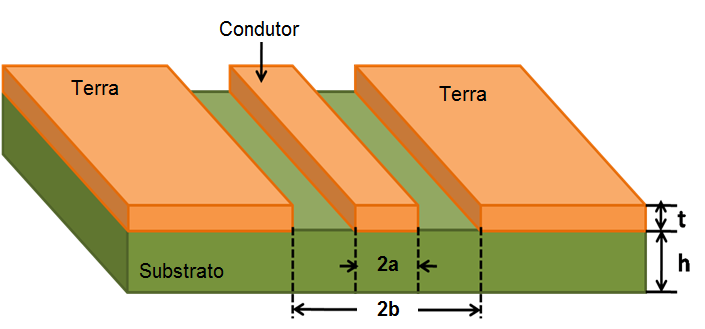
\includegraphics[scale=.5]{./cap1/figuras/coplanar_waveguide.png}
		\caption{Coplanar waveguide}
		\label{fig:CPW}
	\end{center}
\end{figure}
	
Além da estrutura convencional também existem outras formas de CPW que possuem características um pouco diferentes. Entre elas está o \textit{conductor-backed} CPW, ilustrado na figura \ref{fig:backed-CPW}.

\begin{figure}[htb!]
	\begin{center}
		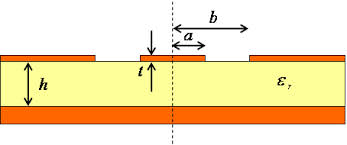
\includegraphics[scale=.6]{./cap1/figuras/backed-CPW.jpg}
		\caption{Conductor-backed coplanar waveguide}
		\label{fig:backed-CPW}
	\end{center}
\end{figure}

As fórmulas utilizadas hoje para a aquisição dos valores de $\varepsilon_{eff}$ e $Z_0$ das estruturas foram derivadas através de métodos de mapeamento conforme (\textit{conformal-mapping}), levando em consideração linhas com espessura zero, e são mostradas a seguir.

Para estruturas coplanares convencionais, segundo \citep{Ghione} temos que:
\begin{equation}
\varepsilon_{eff} = 1+ \frac{\varepsilon - 1}{2}\frac{K(k')}{K(k)}\frac{K(k_1)}{K(k'_1)}
\end{equation}
e 
\begin{equation}
Z_0 = \frac{30\pi}{\sqrt{\varepsilon_{eff}}}\frac{K(k')}{K(k)} 
\end{equation}
onde
\begin{eqnarray}
k &=& \frac{a}{b} \\
k' &=& \sqrt{1-k^2}\\
k_1 &=& \frac{sinh(\pi a/2h)}{sinh(\pi b/2h)}\\
k'_1 &=& \sqrt{1 - k^2_1}
\end{eqnarray}
onde $K(k)$ é a integral elíptica completa de primeira ordem, e seus valores podem ser determinados através da integral ou de através de tabelas.

Devido a importância da integral elíptica de primeira ordem para a análise de vários tipos de linhas de transmissões planares, as equações aproximadas a seguir podem ser utilizadas para o cálculo. [\cite{Hoffmann}]

Para $0 \leq k \leq 0.71$ temos:

\begin{equation}
\label{eq:eliptcal1}
\displaystyle
K(k) = \frac{\pi}{2}\left\lbrace 1+ \frac{2k^2}{8} + \frac{9k^2}{8^2} + 50\left(\frac{k^2}{8}\right)^2 + 306.250\left(\frac{k^2}{8}\right)^4 + ...\right\rbrace
\end{equation}
e para $0.71 <  k \leq 1$
\begin{equation}
\label{eq:eliptcal2}
K(k) = p + \left\lbrace p - 1\right\rbrace\left(\frac{k'^2}{4}\right) + 9\left\lbrace p - \frac{7}{6}\right\rbrace \left(\frac{k'^4}{64}\right) + 25\left\lbrace p - \frac{37}{30}\right\rbrace \left(\frac{k'^6}{256} \right)+ ...
\end{equation}
\begin{equation}
\label{eq:eliptcal3}
p = ln(\frac{4}{k'}) = ln(\frac{4}{\sqrt{1-k^2}})
\end{equation}

O máximo erro relativo das equações \ref{eq:eliptcal1} e \ref{eq:eliptcal2} ocorre o ponto limite $k = \sqrt{0.5} \simeq 0.71$ e é de 3\%. Para $k \rightarrow 0 $ ou $k \rightarrow 1$, o erro relativo em \ref{eq:eliptcal1}, \ref{eq:eliptcal2} e \ref{eq:eliptcal3}, respectivamente, vão para zero. 

Equações simples para a relação $ K(k')/K(k) $ usam projeção estereográfica, definidas por Hilberg, e, para $ 0< k \leq 0.173 $ ou $2 \leq K(k')/K(k) < \infty $, temos as seguintes equações[\cite{Hoffmann}].

\begin{equation}
\label{eq:eliptcal4}
\frac{K(k')}{K(k)} = \left(\frac{4}{\pi} \right) ln\left(\frac{2}{\sqrt{k}}\right)
\end{equation}
\begin{equation}
k = 4 exp\left\lbrace -\frac{\pi K(k')}{2K(k)}\right\rbrace
\end{equation}
e para $ 0.173 < k \leq 1 $ ou $0 \leq K(k')/K(k) < 2 $, temos:
\begin{equation}
\label{eq:eliptcal5}
\frac{K(k')}{K(k)} = \frac{\pi}{ln(2) + 2arctan(\sqrt{k}}
\end{equation}
\begin{equation}
k = \left[tanh\left\lbrace \frac{\pi K(k)}{2K(k') - \frac{ln(2)}{2}}\right\rbrace \right]^2
\end{equation}

O erro relativo para as equações \ref{eq:eliptcal4} e \ref{eq:eliptcal5} é menor que 0.24\%. A função $ K(k')/K(k)$ tende a um valor infinito quando $k=0$, e cai monotonicamente com $k$, chegando a zero quando $k=1$.

A definição completa das integrais elípticas de primeira ordem podem ser encontradas em [\cite{Alan}] e [\cite{Byrd}], Assim como, os resultados também podem ser encontrados já tabelados, como em [\cite{Eugene}]

Quando é levado em consideração a espessura dos condutores, a constante dielétrica efetiva e a impedância característica pode ser calculada da seguinte forma:

\begin{equation}
\displaystyle
\varepsilon_{eff}(t) = \varepsilon_{eff} - \frac{0.7(\varepsilon_{eff}-1)\frac{t}{b-a}}{\frac{K(k)}{K(k')} + 0.7\frac{t}{b-a}}
\end{equation}
e
\begin{equation}
\displaystyle
Z_0 = \frac{30\pi}{\sqrt{\varepsilon_{eff}(t)}}\frac{K(k'_e)}{K(k_e)} 
\end{equation}
onde 
\begin{eqnarray}
\displaystyle
k_e &=& \frac{S_e}{S_e+2W_e}\\
k'_e &=& \sqrt{1 - k^2_e}\\
S_e &=& 2a + \Delta\\
W_e &=& b-a-\Delta\\
\Delta &=&  \frac{1.25t}{\pi} \left[1+\left(\frac{8\pi a}{t}\right)\right]
\end{eqnarray}


\subsection{Microstrip}

Microstrip é uma das formas de estruturas planares mais conhecidas e que é utilizada em diversas aplicações, como antenas e linhas de transmissão dispositivos que trabalhem com RF, principalmente na faixa de ondas milimétricas. Dentre as aplicações de RF mais comuns são as antenas patch, e isso é devido as algumas características que essas estruturas planares possuem, das quais podemos destacar as seguintes:
 \begin{itemize}
 \item Pequena área de ocupação;
 \item Estrutura leve;
 \item Facilidade de fabricação;
 \item Facilidade de  alimentação;
 \item Facilidade para usar em estruturas de array ou em acoplar a outros circuitos microstrip;
 \item Pode assumir qualquer tipo de formato.
 \item Suporta mais de uma frequência de operação.
 \end{itemize}
 
 Porém nem sempre todas as características desse tipo de antenas são vantagens, existem alguns pontos que devem se levados em consideração, como por exemplo a largura de de banda que essas estruturas alcançam, mas que podem ser aumentadas com a utilização de algumas técnicas, ou, por exemplo, quando há a necessidade de isolação do circuito, nesse caso a proteção externa precisa ser considerada.

\begin{figure}[htb!]
	\begin{center}
		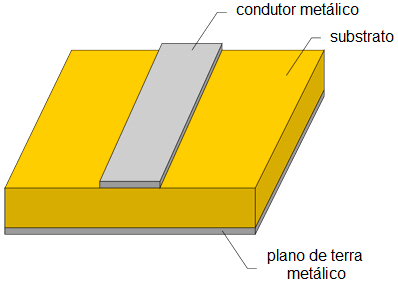
\includegraphics[scale=1]{./cap1/figuras/microstrip.png}
		\caption{Microstrip}
		\label{fig:microstrip}
	\end{center}
\end{figure}

As estrutruas microstrip são  linhas de transmissão geométricas por uma linha condutora simples um dos lados de um substrato dielétrico e um plano de terra simples no lado oposto, como mostrado na figura \ref{fig:microstrip}. Como se trata de uma estrutura aberta, as linhas microstrip tem uma grande vantagem na fabricação comparada com outras estruturas, assim como facilidades para ajustes e interconexões [\cite{Leo}]
%A estruturas microstrip são compostas de uma tira condutora que possui uma largura \emph{w} e espessura \emph{t} e um plano de terra que são separadas por uma camada de material dielétrico (subtrato) de espessura \emph{h} (figura \ref{fig:microstrip}).


A formulas para o cálculo da constante dielétrica efetiva e da impedância característica, hoje já são bem consolidadas, e são mostradas a seguir [\cite{Bhartia}]

\begin{equation}
\varepsilon_{eff} = \frac{\varepsilon_r +1}{2} + \frac{\varepsilon_r -1}{2}\left(1 + \frac{10h}{w}\right)^{-1/2}
\end{equation}
e
\begin{equation}
Z_0 = \frac{42.4}{\sqrt{\varepsilon_r + 1}} ln\left\lbrace 1 + \frac{4h}{w} \left[  G + \sqrt{ G^2 + \frac{\pi^2}{2} \left(  1 + \frac{1}{\varepsilon_r}\right)}\right] \right\rbrace
\end{equation}
onde
\begin{equation}
G =  \left(\frac{14 + \frac{8}{\varepsilon_r}}{11}\right)\frac{4h}{w} 
\end{equation}

\section{Aplicações de Estruturas Planares}

Como já mencionado, as linas de transmissões planares podem ser utilizadas em diversas aplicações devido a suas características físicas, principalmente facilidade de fabricação e integração com outros dispositivos, dentre elas as antenas de micro fita são as mais comuns e são utilizadas nas mais diversas formas de comunicações, em [\cite{Patel}] é foi feito um levantamento de alguns tipos de comunicação que utilização antenas de micro fita, entre elas estão: comunicações móveis, GPS, identificação em radiofrequência (RFID), radar e WiMAx. Mas além de antenas de microfita as estruturas planares também podem ser utilizadas para fabricação de outros dispositivos como anéis de ressonância [\cite{Benjamin}], superfícies seletoras de frequências [\cite{Mauricio}], entre outras.

%Como já mencionado, as linhas planares de transmissão, são muito úteis para algumas aplicações devido as suas características físicas, principalmente pela facilidade de fabricação de tais estruturas. Mas onde tais estruturas podem ser aplicadas para solucionar determinados problemas? Em mutias áreas voltadas para a criação de sistemas, utilizam de alguma forma linhas de transmissões planares, umas das áreas onde mais há esforços a fim de desenvolver tais estruturas é a área de RF, mas especificamente, micro-ondas.

\section{Resumo do Capítulo}

Neste Capítulo buscou mostrar algumas formas de estruturas de transmissões planares que podem ser encontradas hoje, assim como fornecer uma base teórica mínima de como uma estrutura planar pode ser projetada, levando em consideração suas dimensões físicas, como largura da linha de transmissão e a espessura dos dielétricos, assim como mostrar algumas aplicações onde tais estruturas são comumente utilizadas.
%\chapter{Time Domain Reflectometry - TDR \\ (Reflectometria no Domínio do Tempo)}
%\subtitle{Reflectometria no Domínio do Tempo} 
\label{TDR}

O TDR é uma técnica bem conhecida para a análise de sistemas eletrônicos. Ele é tipicamente usado para na caracterização e localização de descontinuidades ou interrupções ao longo de linhas de transmissão de RF[\cite{McCabe}]. O princípio de operação de do TDR funciona similarmente ao Radar, um sinal elétrico é enviado através do sistema medido e quando atinge alguma descontinuidade ou o final do dispositivo retorna com modificações, o que possibilita a identificação das características do sistema. 

\section{Linhas de Transmissão}
Para melhor entendimento de como funciona a medição por meio do TDR um conhecimento sobre linhas de transmissão se faz necessário. Primeiramente, o que é de fato uma linha de transmissão? Uma linha de transmissão nada mais é do que uma conexão física entre dois locais através do uso de um par de condutores, onde as intensidade de campo magnético e campo elétrico são perpendiculares entre si e também perpendicular a direção de propagação[\cite{Ida}]. 

\begin{figure}[htb!]
	\begin{center}
		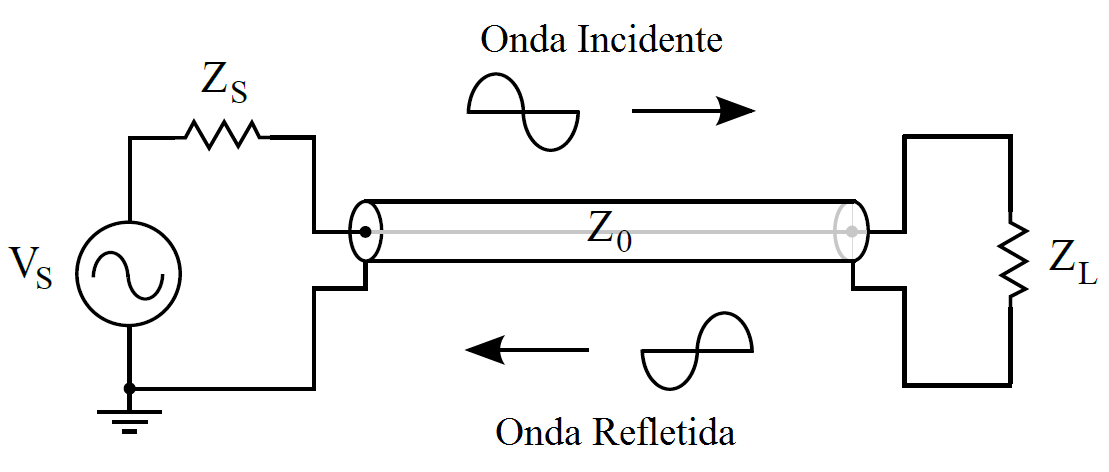
\includegraphics[scale=.4]{./cap2/figuras/incident_reflected.png}
		\caption{Onda incidente e onda refletida em uma linha de transmissão}
		\label{fig:inc_ref}
	\end{center}
\end{figure}

Quando um sinal que está sendo enviado por uma linha de transmissão encontra algum tipo de descontinuidades este então é refletido e segue no sentido oposto ao sinal incidente, como é mostrado na figura \ref{fig:inc_ref}. A velocidade de propagação em uma linha de transmissão pode ser calculada através da equação \ref{eq:velocidade_propagacao}

\begin{equation}
	v_p = \frac{C}{\sqrt{\epsilon_r \mu_r}}
	\label{eq:velocidade_propagacao}
\end{equation}
\noindent
onde \emph{C} é a velocidade de propagação da lu no vácuo, aproximadamente $3.10^8$m/s, $\epsilon_r$ é permissividade relativa do material dielétrico e $\mu_r$ é a permeabilidade relativa do material.

\section{Sistema de Medição}
O sistema para a realização de medições de TDR, é um set-up simples que consiste em um gerador de sinal, que pode ser um degrau ou um impulso, um osciloscópio, que será usado para realizar a leitura do sinal de saída, e o dispositivo a ser medido. O esquemático do sistema de medição é mostrado na figura \ref{fig:circuito_TDR}, onde o sinal do gerador é enviado para o dispositivo em teste através de uma linha de transmissão que possui uma impedância característica $Z_0$, onde convencionalmente o valor assumido dessa impedância é de 50$\Omega$), o sinal após entrar no dispositivo sofre reflexões referentes as descontinuidades e das variações de resistência do dispositivo, este sinal refletido junto com o sinal incidente são então medidos/amostrados pelo osciloscópio pra posteriormente poderem ser analisados

\begin{figure}[htb!]
	\begin{center}
		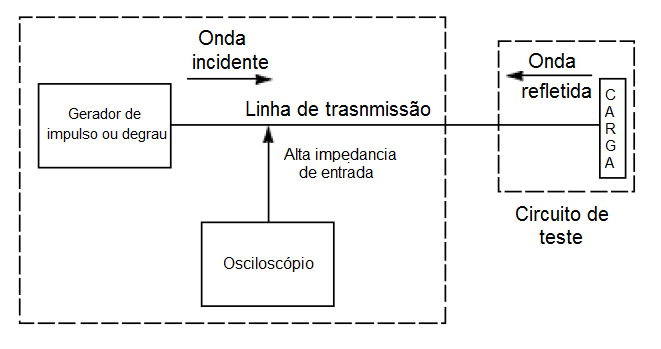
\includegraphics[scale=.6]{./cap2/figuras/simple_TDR.png}
		\caption{Esquema básico para medição TDR}
		\label{fig:circuito_TDR}
	\end{center}
\end{figure}

\section{Sinais de Entrada}

Dois tipos de sinais podem ser utilizados: pulso ou degrau, ambos agem da mesma forma nas medidas, porém, dependo da aplicação em questão uma possui vantagens em relação a outra. A figura \ref{fig:respostas} mostra a resposta para os dois tipos de sinais. O pulso possibilita uma rápida e fácil localização das falhas ou descontinuidades existentes nos sistemas medidos. O degrau também permite uma rápida e fácil localização de falas e descontinuidades, porém, com a vantagem de se obter de forma fácil a impedância no material. Para a pesquisa foi utilizado o degrau que é o sinal utilizado pelo equipamento usado nas medições.

\begin{figure}[htb!]
	\begin{center}
		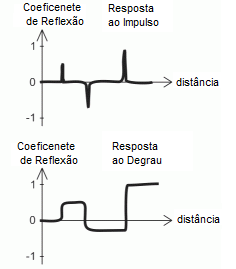
\includegraphics[scale=.9]{./cap2/figuras/tdr_response.png}
		\caption{Respostas típicas para sinais de Pulso e Degrau }
		\label{fig:respostas}
	\end{center}
\end{figure}

Algumas respostas mostradas por esse tipo de medição já são bem conhecidas e equacionadas, entre elas estão a identificação de diferentes impedâncias e os efeitos capacitivos e indutivos que pode aparece ao longo do caminho. Outra resposta é a identificação do final do sistema medido, que pode estar em curto, em aberto ou com alguma carga acoplada nele. 

\section{Amplitude do Sinal Medido}

Para um melhor entendimento será proposto uma modelo simples de medição, onde o que está sendo medido compõe-se de uma linha de transmissão (cabo) e uma carga acoplada ao final, como mostrada na figura \ref{fig:circuito_simples}. A resposta apresentado pelo TDR é uma relação entre a impedância da linha de transmissão e da carga acoplada.

\begin{figure}[htb!]
	\begin{center}
		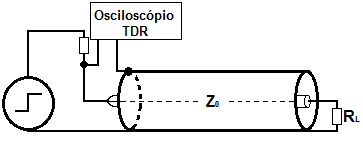
\includegraphics[scale=.7]{./cap2/figuras/simple_circuit_TDR.png}
		\caption{Exemplo de circuito de medição.}
		\label{fig:circuito_simples}
	\end{center}	
\end{figure}

Existem basicamente três casos que podem acontecer: circuito aberto, curto circuito e circuito fechado com carga acoplada; os resultados para cada caso são mostrados na figura \ref{fig:resp_imp}. No caso de circuito aberto a impedância é máxima e o valor mostrado na resposta é a tensão total do pulso incidente. Para para o curto circuito a impedância é mínima logo ocorre o efeito contrario a do circuito aberto, o sinal medido possui valor igual a zero. Já a situação em que há uma carga acoplada no final, podem ocorrer três situações, a primeira é o valor da caga ser igual ao valor da linha de transmissão, assim não havendo mudança no valor medido; a segunda seria com a carga tendo um valor maior que o da linha de transmissão, fazendo com que a diferença entre a relação entre carga e cabo seja positiva; e a terceira e última situação é quando a carga possui valor menor que o cabo, fazendo com que a diferença seja negativa.



\begin{figure}[htb!]
	\begin{center}
		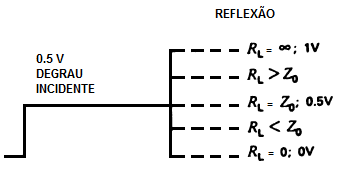
\includegraphics[scale=.7]{./cap2/figuras/resp_impe.png}
		\caption{Resposta para o circuito da figura \ref{fig:circuito_simples}.}
		\label{fig:resp_imp}
	\end{center}	
\end{figure}



\section{Impedância}

Em todo sistema de transmissão um fator físico que sempre deve se levando em consideração é a impedância do sistema. Como já dito o TDR trabalha de forma similar ao radar, onde para cada descontinuidade há uma resposta, mas também mostra a impedância do sistema que é calculado através a amplitude da onda medida. Primeiramente é necessário calcular o coeficiente de reflexão, como mostrado na equação \ref{eq:coe_ref},

\begin{equation}
\rho = \frac{E_r}{E_i} = \frac{R - Z_0}{R + Z_0}
\label{eq:coe_ref}
\end{equation}

Onde $E_r$ é o valor do pulso refletido, $E_i$ é o valor do pulso incidente, $R$ é o valor da carga e $Z_0$ é o valor da impedância da linha de transmissão. Com o valor do coeficiente de reflexão, pode-se deduzir se sistema medido está em curto, aberto ou com alguma carga acoplada. Para isso temos que saber que a quando o valor de $\rho$ = +1 o circuito está aberto, quando $\rho$ = -1, o circuito está em curto, quando $\rho$ = 0 a carga acoplada possui o mesmo valor de impedância que a linha de transmissão, quando 0 < $\rho$ < 1 a carga possui valor maior que a linha de transmissão e quando  -1 < $\rho$ < 0 a carga possui um valor menor, como mostrado na figura \ref{fig:valor_rho}.

\begin{figure}[htb!]
	\begin{center}
		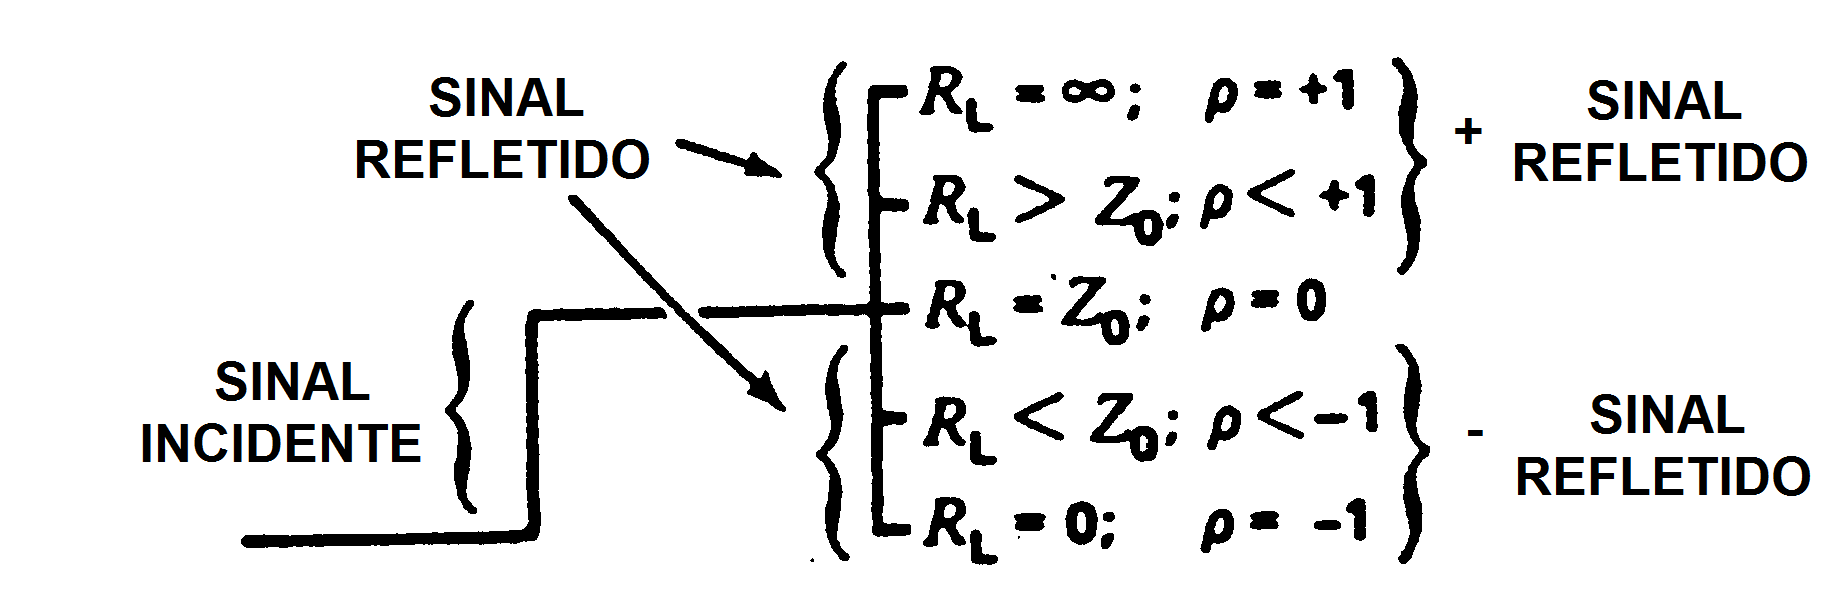
\includegraphics[scale=.18]{./cap2/figuras/tdr_response_reflexao.png}
		\caption{fig:Valores de $\rho$}
		\label{fig:valor_rho}
	\end{center}
\end{figure}

\section{Reflexões Através de Descontinuidades Resistivas}

Dois tipos de reflexões podem ocorrer para dois tipos de descontinuidades resistivas. Eles são uma mudança da reflexão em forma de degrau e uma uma mudança continua da reflexão. Uma resistência em série com uma linha de transmissão causa uma reflexão positiva. A resistência em série com a linha de transmissão causa uma reflexão negativa. Resistores discretos simples causam uma reflexão em degrau, enquanto que resistências distribuídas causa uma mudança contínua. A reflexão para resistores discretos são mostrados de forma ideal na figura \ref{fig:descontinuidade_resistor_simples} e a reflexão para resistência distribuída é mostrada de forma ideal na figura \ref{fig:descontinuidade_resistor_distribuido}.

\begin{figure}[htb!]
	\begin{center}
		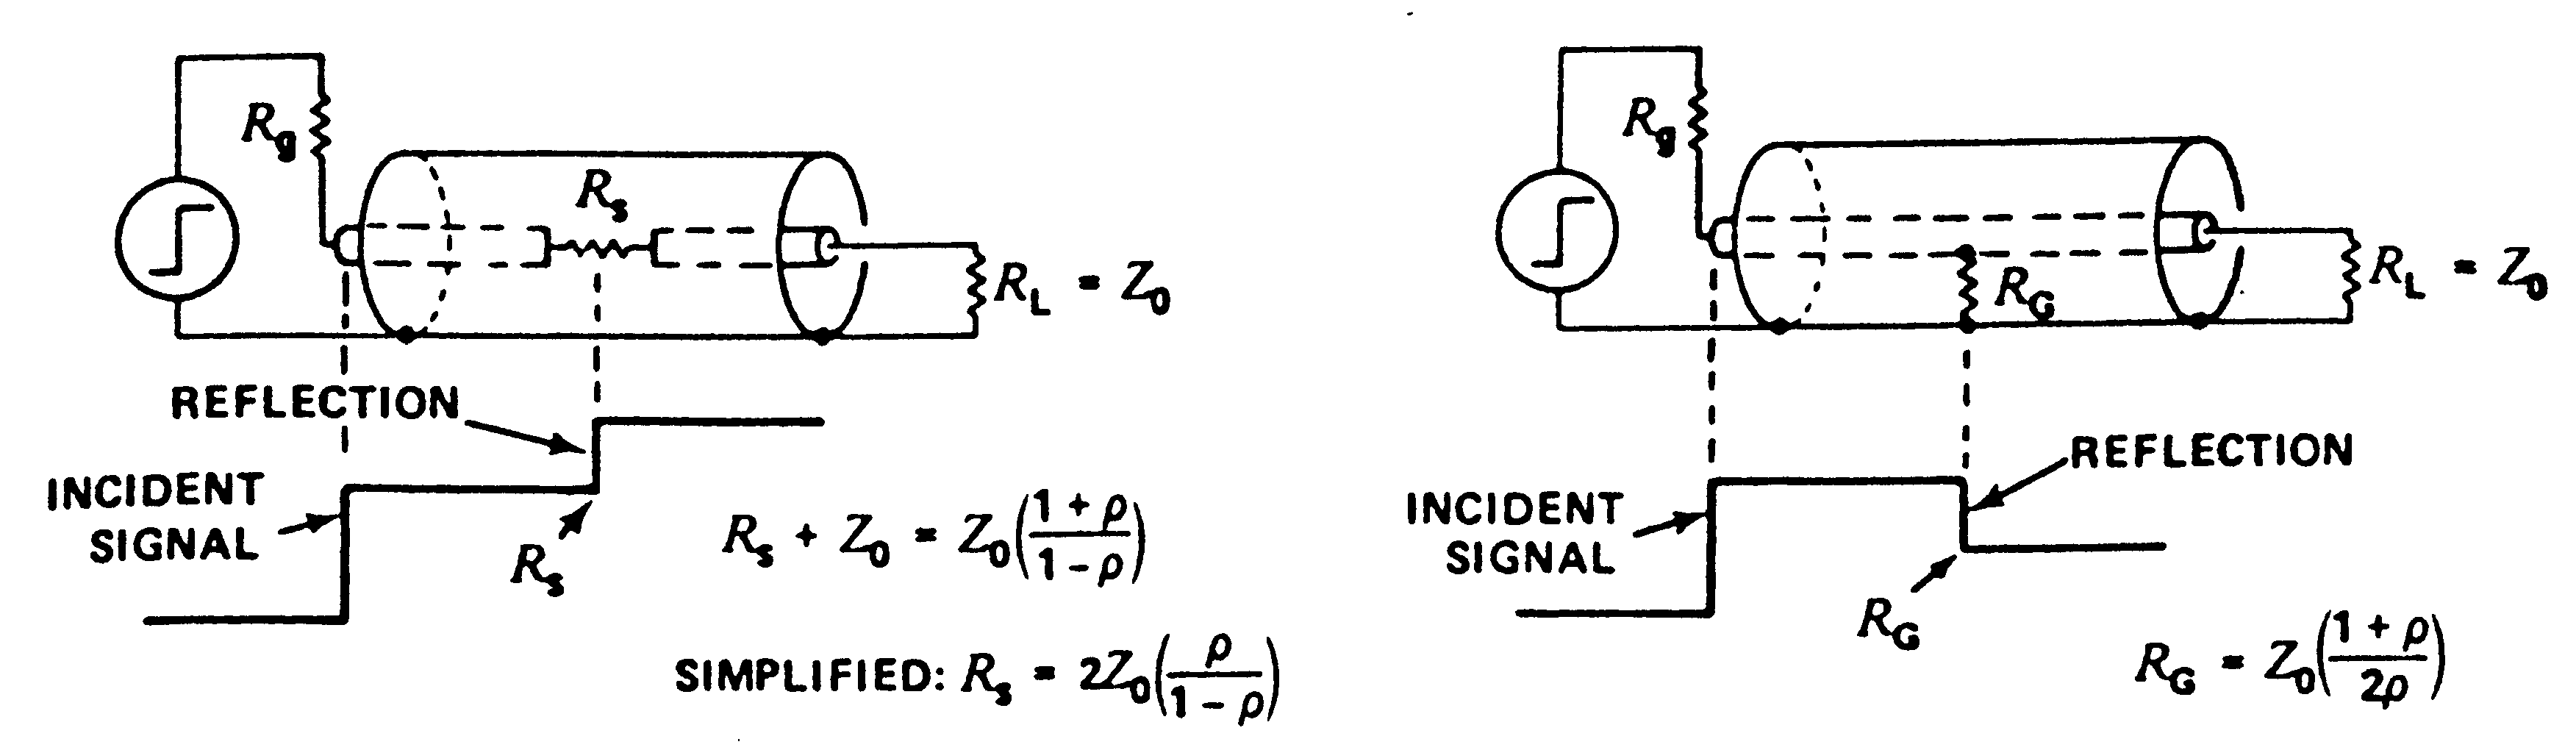
\includegraphics[scale=.15]{./cap2/figuras/discontinuidade_resistor_simples.png}
		\caption{Descontinuidades de Resistores simples e suas reflexões}
		\label{fig:descontinuidade_resistor_simples}
	\end{center}
\end{figure}

\begin{figure}[htb!]
	\begin{center}
		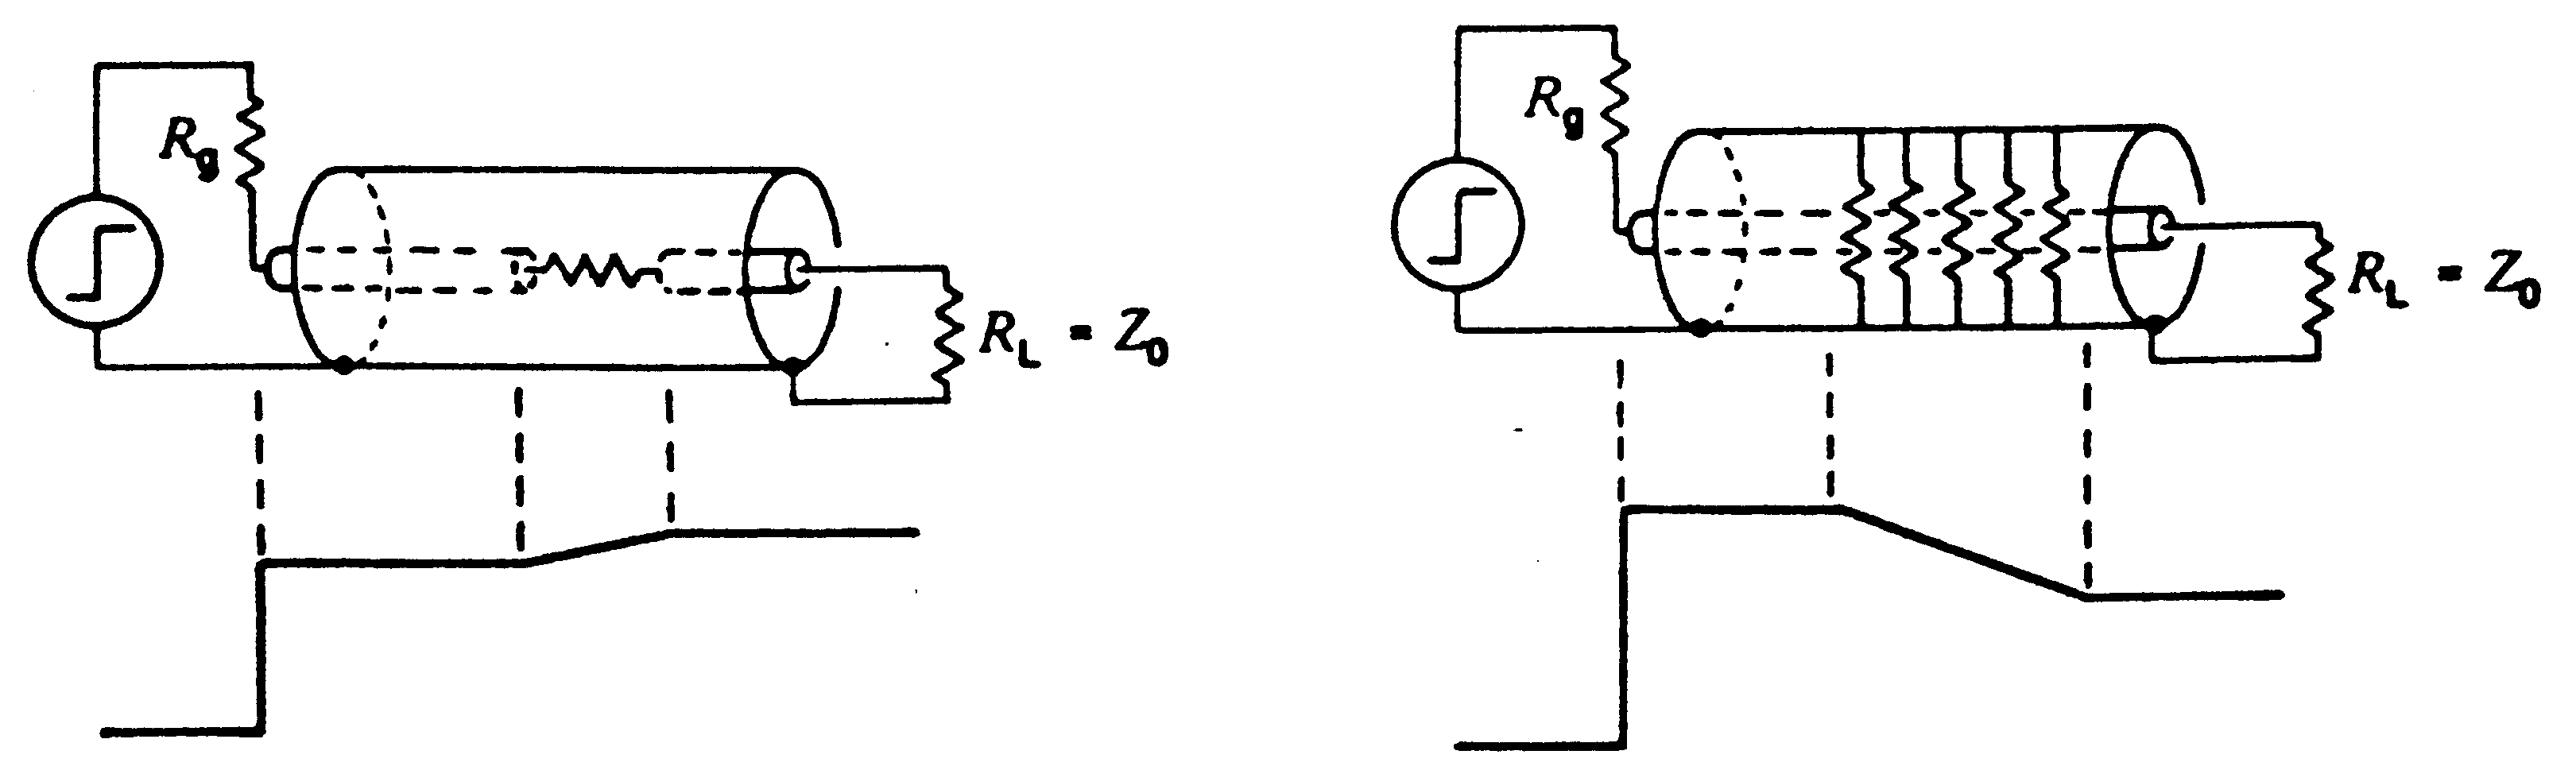
\includegraphics[scale=.15]{./cap2/figuras/discontinuidade_resistor_distrubuido.png}
		\caption{Descontinuidade de resistência distribuída e suas reflexões}
		\label{fig:descontinuidade_resistor_distribuido}
	\end{center}
\end{figure}

A figura \ref{fig:descontinuidade_resistor_distribuido} mostra de forma me exagerada o começo da resistência distribuída em um ponto particular da linha. Normalmente, tando resistência em série quanto em paralelo são encontradas ao longo de toda a extensão de qualquer cabo coaxial testado.

As quatro formas de são uma indicação de perda de sinal entre a entrada e a saída de uma linha de transmissão. A descontinuidade de uma resistor simples pode ocorrer para componentes discretos como um conector solto com adição de uma resistência em série. Tais descontinuidades podem ser localizados fisicamente pelo TDR. Perdas distribuídas são usualmente partes particulares de uma linha que está sendo testada e o display do TDR pode mostrar um valor para uma análise quantitativa de resistência por unidade de tamanho. [\cite{TDK}]
\section{Cargas Capacitivas e Indutivas}

Ao final do sistema medido também podem ser encontradas cargas que nãos seja apenas da resistivas, mas também capacitivas ou indutivas que podem ser encontradas em 2 configurações cada, em série ou em paralelo. Os elementos capacitivos e indutivos possuem comportamentos bem definidos, a seguir são mostrados as respostas para capacitores acoplados.

\begin{figure}[htb!]
	\begin{center}
		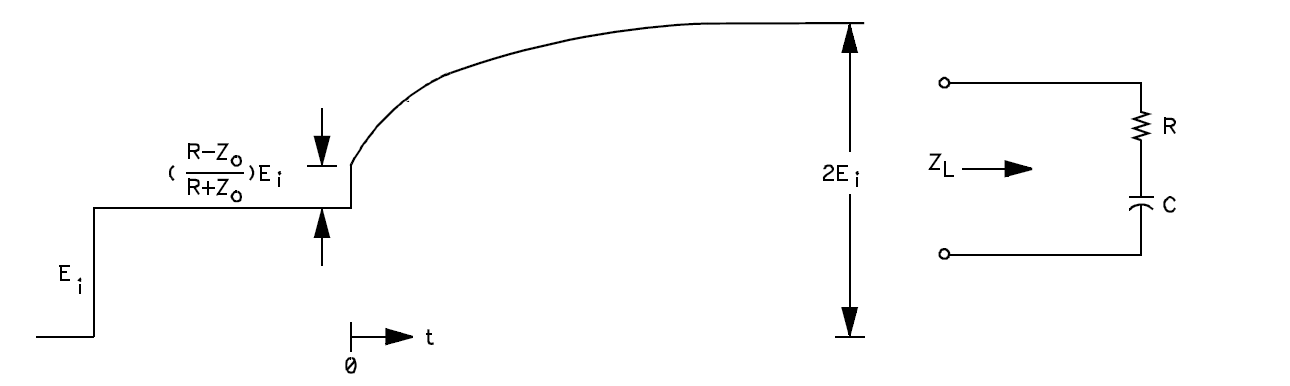
\includegraphics[scale=.30]{./cap2/figuras/R-C_serie_response.png}
		\caption{Circuito R-C em serie}
		\label{fig:RC_serie}
	\end{center}
\end{figure}

\begin{figure}[htb!]
	\begin{center}
		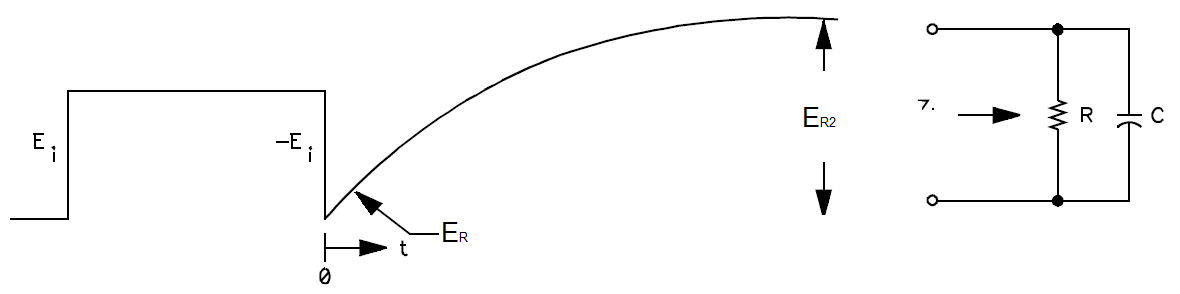
\includegraphics[scale=.30]{./cap2/figuras/R-C_parallel_response.png}
		\caption{Circuito R-C em Paralelo}
		\label{fig:RC_paralelo}
	\end{center}
\end{figure}

Na figura \ref{fig:RC_serie}, a curva de subida do gráfico é pode ser expressa pela equação \ref{eq:RC_serie}.

\begin{equation}
\label{eq:RC_serie}
E_R = E_i\left[(2 - \left(1-\frac{R-z_0}{R+z_0}e^{\frac{-t}{\tau}}\right)\right] \\
\end{equation}

\begin{equation}
\tau = (Z_0+R)C
\end{equation}

E na figura \ref{fig:RC_paralelo}, a curva de subida é dada pelas equações \ref{eq:RC_paralelo} e \ref{eq:RC_paralelo_estacionario}

\begin{equation}
\label{eq:RC_paralelo}
E_R = E_i\left[\left( 1 + \frac{R-Z_0}{R+Z_0}\right)\left( 1 - e^{\frac{-t}{\tau}}\right)\right]
\end{equation}

\begin{equation}
\label{eq:RC_paralelo_estacionario}
E_{R2} = E_i \left(1+ \frac{R-Z_0}{R + Z_0}\right)
\end{equation}

\begin{equation}
\tau = \frac{Z_0R}{Z_0+R}C
\end{equation}

Para a situação da figura \ref{fig:RC_paralelo}, no tempo zero, a carga aparece como um circuito aberto, uma vez que o capacitor não aceita uma repentina repentina de tensão. Portanto $\rho = -1$ quando $t =0$. Após uma espaço de tempo, entretanto, a voltagem em C aumenta e a sua impedância cresce. Em $ t = \inf$, o capacitor torna-se uma circuito aberto. Uma análise semelhante também pode ser feita para a situação apresentada na figura \ref{fig:RC_serie}.[\cite{agilent}]

Para caragas como indutores acopladas ao final do sistemas temos um tipo de resposta diferente que são mostradas nas figuras \ref{fig:RL_serie} e \ref{fig:RL_paralelo}.

\begin{figure}[htb!]
	\begin{center}
		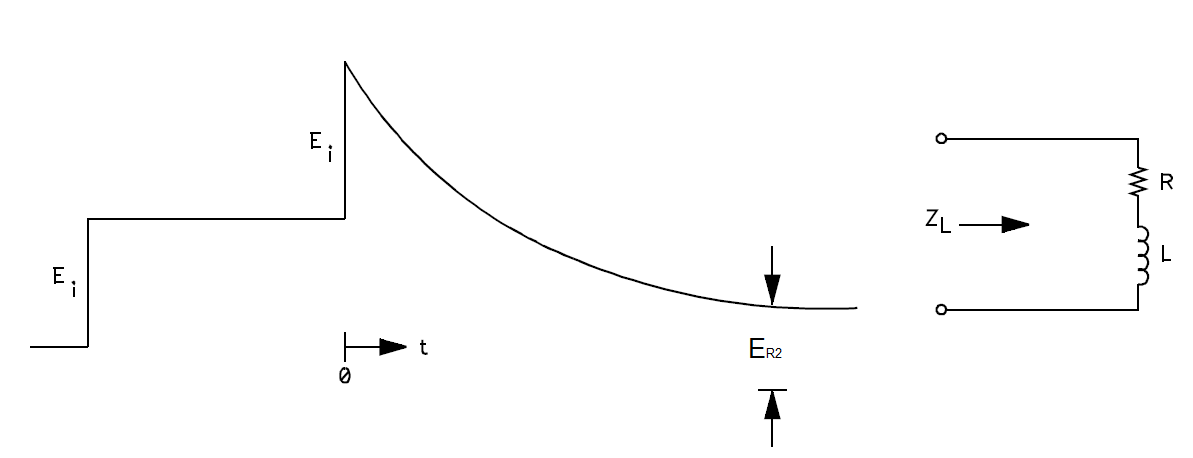
\includegraphics[scale=.30]{./cap2/figuras/R-L_serie_response.png}
		\caption{Circuito R-L em serie}
		\label{fig:RL_serie}
	\end{center}
\end{figure}

\begin{figure}[htb!]
	\begin{center}
		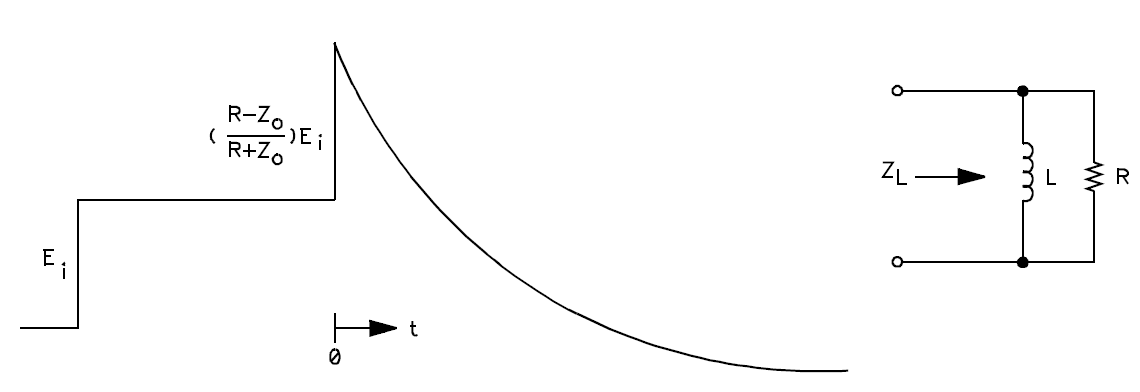
\includegraphics[scale=.30]{./cap2/figuras/R-L_parallel_response.png}
		\caption{Circuito R-L em Paralelo}
		\label{fig:RL_paralelo}
	\end{center}
\end{figure}

A curva de descida mostrada na figura \ref{fig:RL_serie} é definida pelas equações \ref{eq:RL_serie} e \ref{eq:RL_serie_estacionario}.
%
\begin{equation}
\label{eq:RL_serie}
E_R = E_i \left[\left( 1 + \frac{R - Z_0}{R + Z_0}\right) + \left( 1 + \frac{R - Z_0}{R + Z_0}\right) e^{\frac{-t}{\tau}}\right]
\end{equation}

\begin{equation}
\label{eq:RL_serie_estacionario}
E_{R2} =  E_i \left( 1 + \frac{R - Z_0}{R + Z_0}\right) 
\end{equation}

\begin{equation}
\label{eq:tau_RL}
\tau = \frac{L}{R + Z_0}
\end{equation}

E para a situação mostrada na figura \ref{fig:RL_paralelo}, a cura de descida pode ser expressa pela equação \ref{eq:RL_paralelo}.

\begin{equation}
\label{eq:RL_paralelo}
E_R = E_i\left[\left( 1 + \frac{R-Z_0}{R+Z_0}\right)e^{\frac{-t}{\tau}}\right]
\end{equation}


\begin{equation}
\tau = \frac{Z_0+R}{Z_0R}L
\end{equation}

Para o caso mostrado na figura \ref{fig:RL_serie}, no tempo $t = 0$ a tensão refletida é $+E_i$. Isso ocorre porque o indutor não aceita uma mudança repentina na corrente; assim inicialmente comportando-se como uma impedância infinita, e $\rho = +1$ para $t = 0$. Então a corrente aumenta exponencialmente e sua impedância cai para zero. Quando $t \rightarrow \infty$ então $e_r(t)$ é definido somente pelo valor de R. [\cite{agilent}]
O exponencial de transição de $e_r(t)$ tem uma constante de tempo determinada pelar resistência efetiva vista pelo indutor, mostrado na equação \ref{eq:tau_RL}. Uma análise semelhante também pode ser feita para a figura \ref{fig:RL_paralelo}.

Capacitores e indutores também podem aparecer como descontinuidades na linha de transmissão, geralmente elas aparecem em uma forma bem simples, na forma de pequenas ondas, como ilustrado nas figuras \ref{fig:descontinuidade_C_L} e \ref{fig:Descontinuidade_CL}.


\begin{figure}
	\begin{center}
		 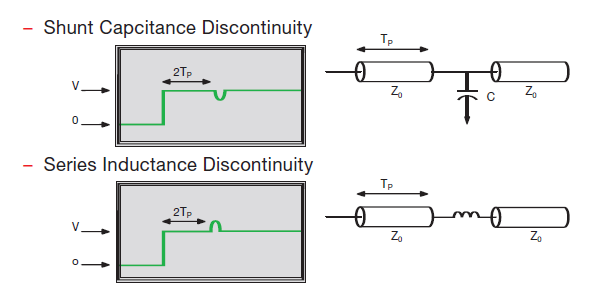
\includegraphics[scale=.5]{./cap2/figuras/C_L_descontinuidade.png}
		 \caption{Descontinuidades capacitivas e descontinuidade indutivas.[\cite{TDK2}]}
		 \label{fig:descontinuidade_C_L}
	\end{center}
\end{figure}


\begin{figure}
	\begin{center}
		 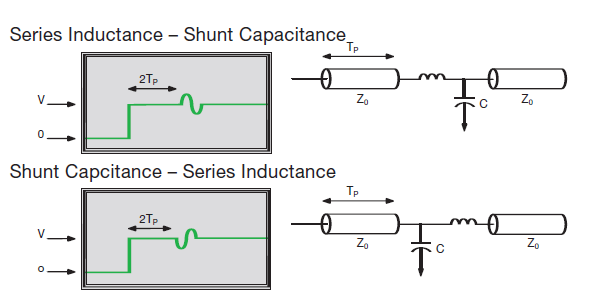
\includegraphics[scale=.5]{./cap2/figuras/CL_descontinuidade.png}
		 \caption{Descontinuidade capacitiva e indutiva. [\cite{TDK2}]}
		 \label{fig:Descontinuidade_CL}
	\end{center}
\end{figure}


\section{Localização de Descontinuidades}

Para a localização da distância da descontinuidade deve-se ter em mão o valor da velocidade de propagação do sinal que é dado por:

\begin{equation}
v_p = \frac{\omega}{\beta} 
\end{equation}
 
ou

\begin{equation}
v_p = \frac{c}{\sqrt{\varepsilon_r}}
\end{equation}

Onde $c$ é a velocidade da luz e $\varepsilon$ é a constante dielétrica do da linha de transmissão. A distancia de propagação é dada por:

\begin{equation}
d = v_pt
\end{equation}

logo 

\begin{equation}
\label{eq:distancia}
d = \frac{c}{\sqrt{\varepsilon_r}}\frac{t_0}{2}
\end{equation}

Onde $t_0$ é a variação do tempo entre o pulso incidente e o pulso refletido. O tempo aparece dividido por dois, pois deve-se levar em consideração que a distancia que o pulso percorre para chegar à descontinuidade e voltar. Dessa forma também podemos calcular a distância entre duas descontinuidades, que é dada por:

\begin{equation}
\Delta d = \frac{c}{\sqrt{\varepsilon_r}}\frac{t_2 - t_1}{2}
\end{equation}

onde $t_1$ é o tempo de viagem nos dois sentidos até a primeira descontinuidade e $t_2$ é o tempo de viagem nos dois sentidos até a segunda descontinuidade. Essas duas descontinuidades podem se tornar indistinguíveis quando separadas por um tempo ($t_2 - t_1$) de metade do tempo de subida do pulso do sistema. Dessa maneira a menor distância para se distinguir duas descontinuidades é dado por 

\begin{equation}
d_{min} = \frac{c}{\sqrt{\varepsilon_r}}\frac{t_r}{4}
\end{equation}

Isso significa que um sistema que possui um tempo de subida de 45ps, duas descontinuidades se juntam e tornam-se indistinguíveis a uma distancia de 3.5mm, utilizando-se o ar como dielétrico. [\cite{agilent}]

\section{Aplicações}

\section{Resumo do Capítulo}

Neste capítulo foi fornecido toda a base teórica necessária para a realização da medição e a análise dos resultado obtidos através do Método de TDR, assim como também mostrar como ele pode ser útil para a aquisição de outros tipos de dados, além apenas da impedância característica do sistema.


%
%\include{cap2}

%\include{resultados}
%
%
%\chapter*{Conclusões Preliminares}
\addcontentsline{toc}{chapter}{Conclusões Preliminares}
O método de medição TDR, mostra-se com uma ferramenta de grande valia quando se trada da avaliação de sistemas, possibilitando a sua utilização em diversas áreas de aplicação, tanto em telecomunicações quanto em monitoramentos. Essa característica se dá pela relativa simplicidade de medição e interpretação dos dados por ela mostrados. 

Nessa avaliação inicial está sendo levando em consideração apenas o aspecto quantitativo de análise. O TDR mostrou-se de grande valia por conseguir distinguir diferentes partes da antena, assim como a possibilidade de poder fazer uma classificação do tipo de respostas que cada tipo de antena pode mostrar, dessa forma facilitando de identificação de estruturas utilizadas da confecção de cada antena e definir sua assinatura elétrica. Com esses resultados iniciais também foi possível fazer a identificação de alguns problemas que podem ocorrer e que afetam a medição para o projeto proposto, como foi o caso do plano de terra, que por ele não possuir um comprimento maior ou igual ao comprimento da antena em questão, não foi possível fazer a caracterização completa da antena.

\section*{Próximas Etapas}
\addcontentsline{toc}{section}{Próximas Etapas}
Para o decorrer da pesquisa está previsto a realização de novas medições em estruturas diferentes, assim como também o equacionamento do padrão de resposta de algumas estruturas, como por exemplo a estrutura de meandro, apresentada nos resultados parciais. Serão investigadas também outras técnicas tais como: TDR diferencial e FDR (Frequency Domain Reflectometry).

Estamos avaliando a possibilidade de caracterização de segmentos planares através da \textbf{matriz-Z}, em seguimentos retangulares a princípio, ou por outros métodos como o \textbf{método das cavidades} ou \textbf{método dos momentos}(\cite{Gupta}).

Estruturas mais complexas, como módulos de transmissão e recepção (T-R modules) e estruturas de array planar, também poderão ser analisadas.


%\cite{McCarb}, \cite{Bhartia} , \cite{Cataldo}



%=============================== Bibliografia ===============================================
\addcontentsline{toc}{chapter}{Bibliografia}
\renewcommand{\bibname}{Bibliografia}
\markboth{Bibliografia}{Bibliografia}

\bibliographystyle{plainnat}
\bibliography{./Referencias/ref}

\end{document}
